\documentclass[brazil,aspectratio=169]{beamer}
\usepackage[utf8]{inputenc}
\usepackage{hyperref}
\hypersetup{
  colorlinks   = true, %Colours links instead of ugly boxes
  urlcolor     = blue, %Colour for external hyperlinks
  linkcolor    = blue, %Colour of internal links
  citecolor   = red %Colour of citations
}

%Inner and Outer themes
\useinnertheme[shadow=true]{rounded}
\useoutertheme{shadow}
\useoutertheme{infolines}

%Custom colors
\definecolor{my-green}{RGB}{183,219,132}
\definecolor{my-blue}{RGB}{50,110,172}
\definecolor{light-black}{RGB}{51,51,51}

\definecolor{terminal-black}{RGB}{48,10,36}
\definecolor{terminal-white}{RGB}{255,255,254}
\definecolor{terminal-gray}{RGB}{223,215,207}

%Inner color
\setbeamercolor{structure}{fg=my-blue,bg=my-green}
\setbeamercolor{section name}{fg=white,bg=my-blue!75!black}
\setbeamercolor{block title}{fg=white,bg=my-blue!75!black}
\setbeamercolor{block title alerted}{use=alerted text,fg=white,bg=alerted text.fg!75!black}
\setbeamercolor{block title example}{fg=terminal-black,bg=terminal-gray!75!white}
\setbeamercolor{block body}{parent=normal text, bg=my-green!10!bg}
\setbeamercolor{block body alerted}{parent=normal text,use=block title alerted,bg=block title alerted.bg!10!bg}
\setbeamercolor{example text}{fg=terminal-white}
\setbeamercolor{block body example}{parent=example text, bg=terminal-black}

%Outer color
\setbeamercolor{palette primary}{fg=white,bg=my-blue}
\setbeamercolor{palette secondary}{fg=white,bg=my-blue!75!black}
\setbeamercolor{palette tertiary}{fg=white,bg=my-green!50!black}
\setbeamercolor{palette quaternary}{fg=white,bg=black}
\setbeamercolor{titlelike}{parent=palette primary}
\setbeamercolor{separation line}{}
\setbeamercolor{fine separation line}{}
\setbeamercolor{author in head/foot}{parent=palette tertiary}
\setbeamercolor{title in head/foot}{parent=palette secondary}
\setbeamercolor{date in head/foot}{parent=palette primary}

\title[Git]{Aprenda a gerenciar seu projeto com o Git.}
\author[L. C. M. de Aquino]{
  Prof. Me. Luiz C. M. de Aquino. \\
}
\institute[DCEX/UFVJM]{
 Universidade Federal dos Vales do Jequitinhonha e Mucuri.\\
 Departamento de Ciências Exatas. \\
 Teófilo Otoni, MG.
}
\date{Outubro, 2020}
%\logo{\includegraphics[scale=0.5]{logo/lncc.eps}}

\newcommand{\terminal}[1]{\textcolor{my-green}{\texttt{#1}}}

\begin{document}

\frame{
\begin{center}
  Semana Nacional de Ci\^encia e Tecnologia do IFNMG \& UFVJM 2020: 
  criando um ambiente de inova\c c\~ao.
\end{center}
\titlepage}

\begin{frame}{Roteiro}

\tableofcontents{}
\end{frame}

\section{Conceitos Básicos.}
\begin{frame}{Controle de Versão}

\begin{block}{\ }
\begin{itemize}
 \item É um sistema que gerencia as mudanças feitas em um conjunto de documentos;
 \item Cada mudança é identificada por um código (``número da revisão''). Por exemplo, um conjunto inicial de arquivos é a 
 ``revisão 1''. Após efetuar algumas mudanças nesses arquivos, temos a ``revisão 2'' e assim sucessivamente;
 \item Cada mudança é associada ao tempo que foi realizada e a pessoa que realizou;
 \item As revisões podem ser comparadas, restauradas ou mescladas.
\end{itemize}
\end{block}

\begin{figure}
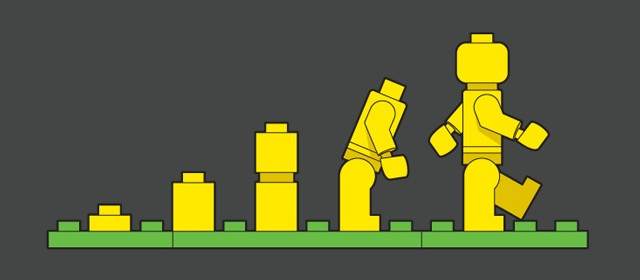
\includegraphics[scale=0.35]{imagens/control-version}
\end{figure}
\end{frame}

\begin{frame}{Arquitetura.}
\begin{figure}
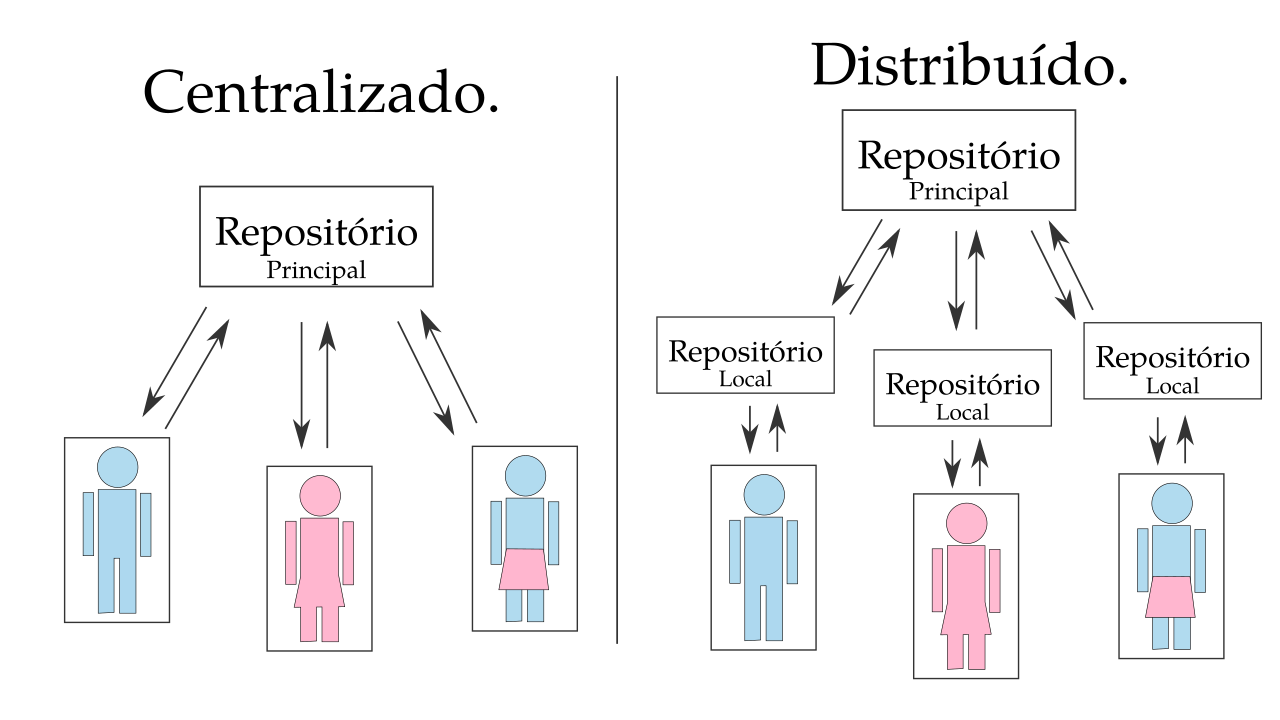
\includegraphics[scale=0.35]{imagens/arquitetura}
\end{figure}
\end{frame}

\begin{frame}{Colaboração.}
\begin{figure}
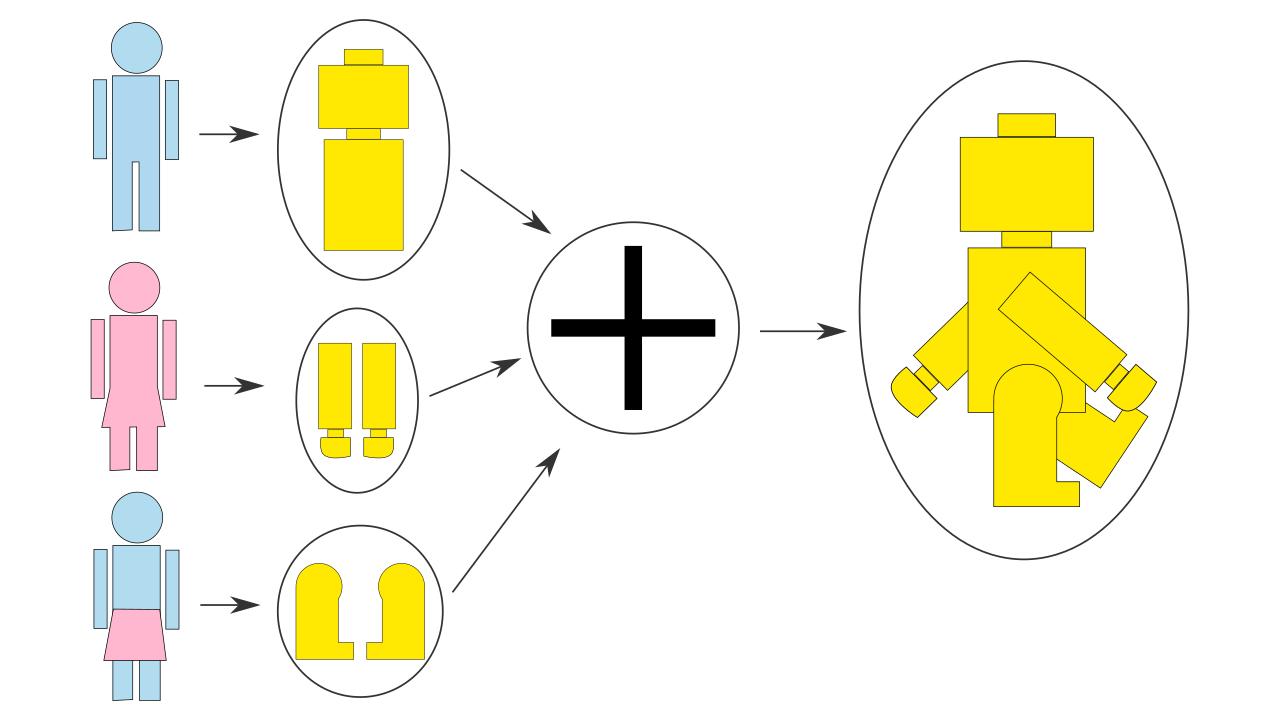
\includegraphics[scale=0.35]{imagens/colaboracao}
\end{figure}
\end{frame}

\begin{frame}{Ferramentas.}
\begin{figure}

\includegraphics[scale=0.35]{imagens/ferramentas}
\end{figure}
\end{frame}

\begin{frame}{Interesse no Git.}

  \begin{figure}
    \centering
    Interesse pelo Git nos últimos 5 anos.   
    
    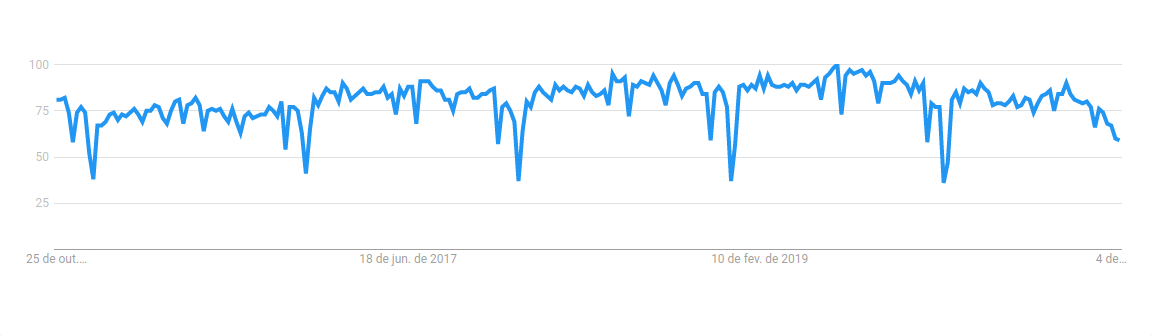
\includegraphics[scale=1]{imagens/git-trends-google}	   
    
    \url{https://trends.google.com/}
  \end{figure}

\end{frame}

\section{Características do Git.}
\begin{frame}{O Git.}
\begin{figure}
  \centering
  
\includegraphics[scale=0.35]{imagens/git-logo}
  
  \url{https://git-scm.com/}
\end{figure}

\begin{block}{\ }
\begin{itemize}
 \item Criado por Linus Torvalds em 2005;
 \item Sistema Distribuído;
 \item Compatível com outros sistemas;
 \item Permite desenvolvimento não linear;
 \item Leve, rápido, confiável e seguro;
 \item Livre;
 \item Usado por empresas como Google, Facebook e Netflix.
\end{itemize}
\end{block}

\end{frame}

\begin{frame}{O GitHub.}
\begin{figure}
  \centering
  
\includegraphics[scale=0.35]{imagens/github-logo}

  \url{http://www.github.com}
\end{figure}

\begin{block}{\ }
\begin{itemize}
 \item GitHub é uma versão baseada em Web do Git. Ele foi lançado em 2008 e comprado
 pela Microsoft em 2018 por US\$ 7,5 bilhões;
 \item Qualquer pessoa pode se registrar gratuitamente;
 \item Oferece a hospedagem de projetos públicos ou privados;
 \item Tem mais de 36 milhões de usuários e 100 milhões de repositórios;
 \item É o maior repositório mundial de código.
\end{itemize}
\end{block}
\end{frame}

\begin{frame}{Git + GitHub.}
\begin{figure}
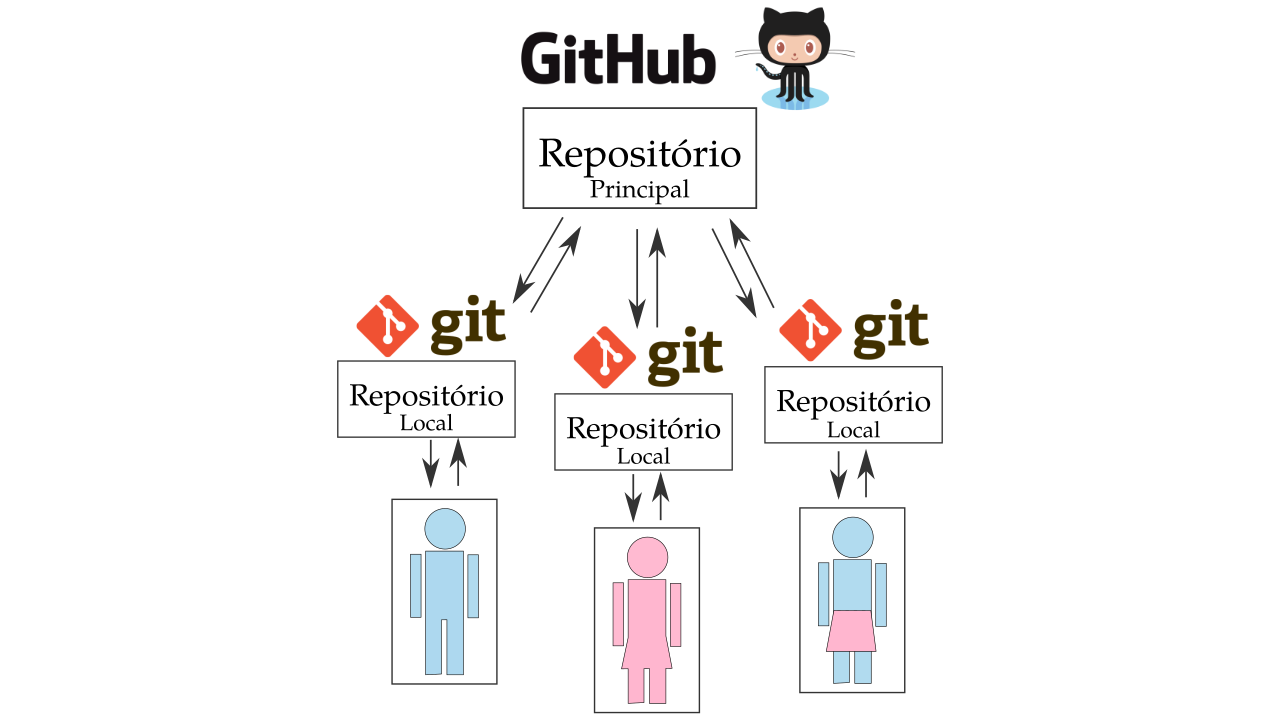
\includegraphics[scale=0.35]{imagens/git_e_github}
\end{figure}
\end{frame}

\section{Operações e Comandos do Git.}
\begin{frame}{Iniciar um repositório.}

\begin{exampleblock}{Terminal}
\~\,\$ \terminal{mkdir meu-repositorio}

\~\,\$ \terminal{cd meu-repositorio}

\~\,\$ \terminal{git init}

Initialized empty Git repository in /meu-repositorio/.git/

\end{exampleblock}

Será criada uma pasta ``.git'' dentro de ``meu-repositorio''.

\end{frame}

\begin{frame}{Adicionar arquivos.}

Crie os arquivos ``programa.cpp'', ``minhaclasse.cpp'' e ``minhaclasse.h''. Em seguida, imprima o \textit{status}
do repositório.

\begin{exampleblock}{Terminal}
\~\,\$ \terminal{git status}

No ramo master

No commits yet

Arquivos não monitorados:

  (utilize ``git add $<$arquivo$>$...'' para incluir o que será submetido)
  
	minhaclasse.cpp
	
	minhaclasse.h
	
	programa.cpp

nada adicionado 
\end{exampleblock}
\end{frame}

\begin{frame}{Adicionar arquivos.}

Para adicionar um arquivo específico, usamos o comando abaixo.

\begin{exampleblock}{Terminal}
\~\,\$ \terminal{git add programa.cpp}
\end{exampleblock}

Já para adicionar todos os arquivos, usamos o seguinte comando.

\begin{exampleblock}{Terminal}
\~\,\$ \terminal{git add -A}
\end{exampleblock}
\end{frame}

\begin{frame}{Adicionar arquivos.}

Vejamos o \textit{status} do repositório novamente.

\begin{exampleblock}{Terminal}
\~\,\$ \terminal{git status}

No ramo master

No commits yet

Mudanças a serem submetidas:

(utilize ``git rm --cached $<$arquivo$>$...'' para não apresentar)

new file:   minhaclasse.cpp

new file:   minhaclasse.h

new file:   programa.cpp
\end{exampleblock}

\end{frame}

\begin{frame}{Salvar as mudanças.}

  Antes de salvar as mudanças no repositório precisamos identificar o autor delas.

  \begin{exampleblock}{Terminal}
    \~\,\$ \terminal{git config user.email "contato@professoraquino.com.br"}

    \~\,\$ \terminal{git config user.name "Luiz C. M. de Aquino"}
  \end{exampleblock}

\end{frame}

\begin{frame}{Salvar as mudanças.}

Para salvar todas as mudanças no repositório usamos o comando abaixo.

\begin{exampleblock}{Terminal}
\~\,\$ \terminal{git commit -m "Criando os arquivos iniciais."}

[master (root-commit) ac7efeb] Criando os arquivos iniciais.

3 files changed, 20 insertions(+)

create mode 100644 minhaclasse.cpp

create mode 100644 minhaclasse.h

create mode 100644 programa.cpp
 
\end{exampleblock}
\end{frame}

\begin{frame}{Verificar o histórico.}

  Para verificar o histórico das mudanças usamos o comando abaixo.

  \begin{exampleblock}{Terminal}
    \~\,\$ \terminal{git log}

    commit ac7efebfcb22d61414f993b1e755a053d4ef7b88 (HEAD -$>$ master)

    Author: Luiz C. M. de Aquino $<$contato@professoraquino.com.br$>$

    Date: Fri Out 23 08:00:00 2020 -0300

    Criando os arquivos iniciais.
  \end{exampleblock}
  
\end{frame}

\begin{frame}{Criar um repositório remoto.}

Vamos criar um repositório central no GitHub para receber o nosso projeto.

\begin{figure}
 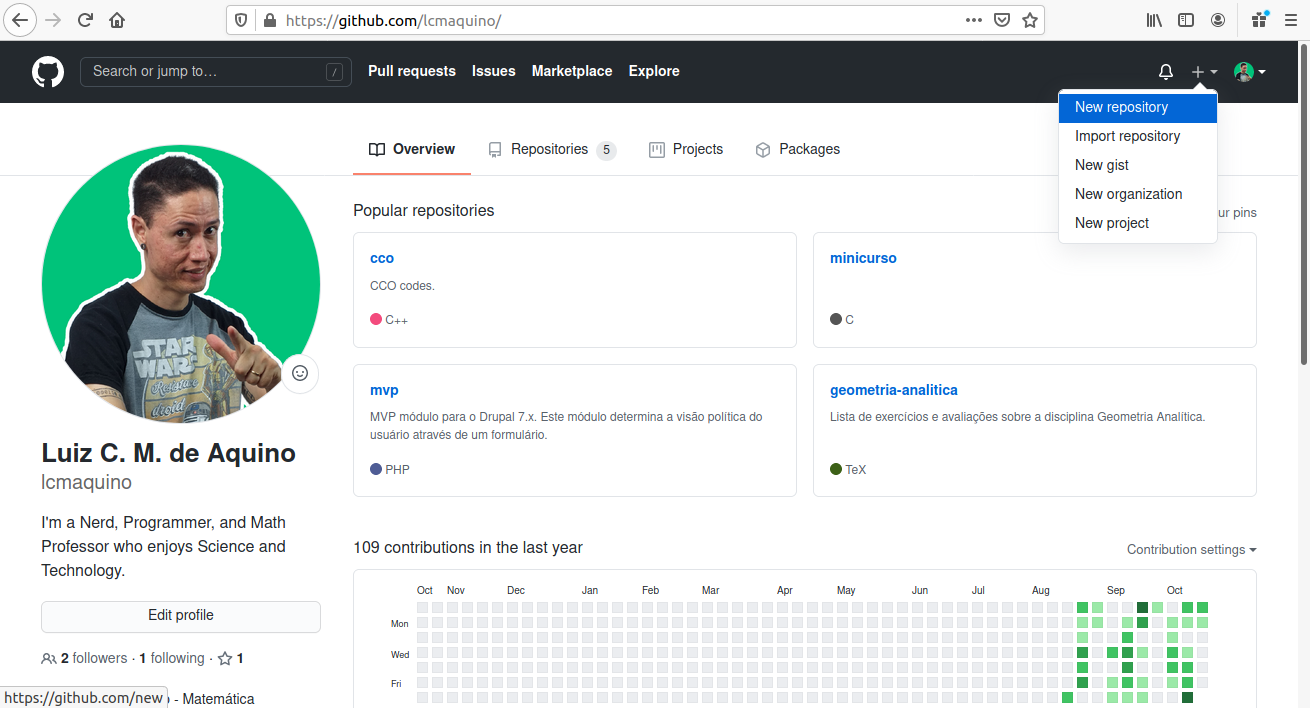
\includegraphics[scale=0.3]{imagens/novo-repositorio-github-1}
\end{figure}
\end{frame}

\begin{frame}{Criar um repositório remoto.}

\begin{figure}
 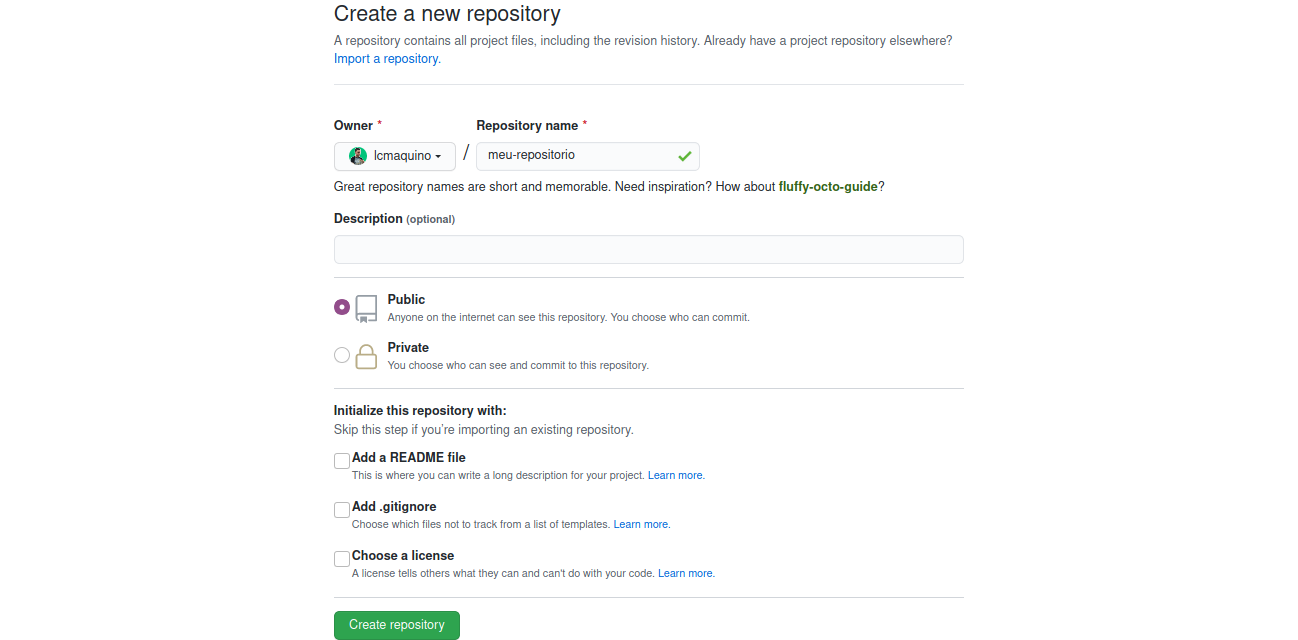
\includegraphics[scale=0.3]{imagens/novo-repositorio-github-2}
\end{figure}
\end{frame}

\begin{frame}{Criar um repositório remoto.}

\begin{figure}
 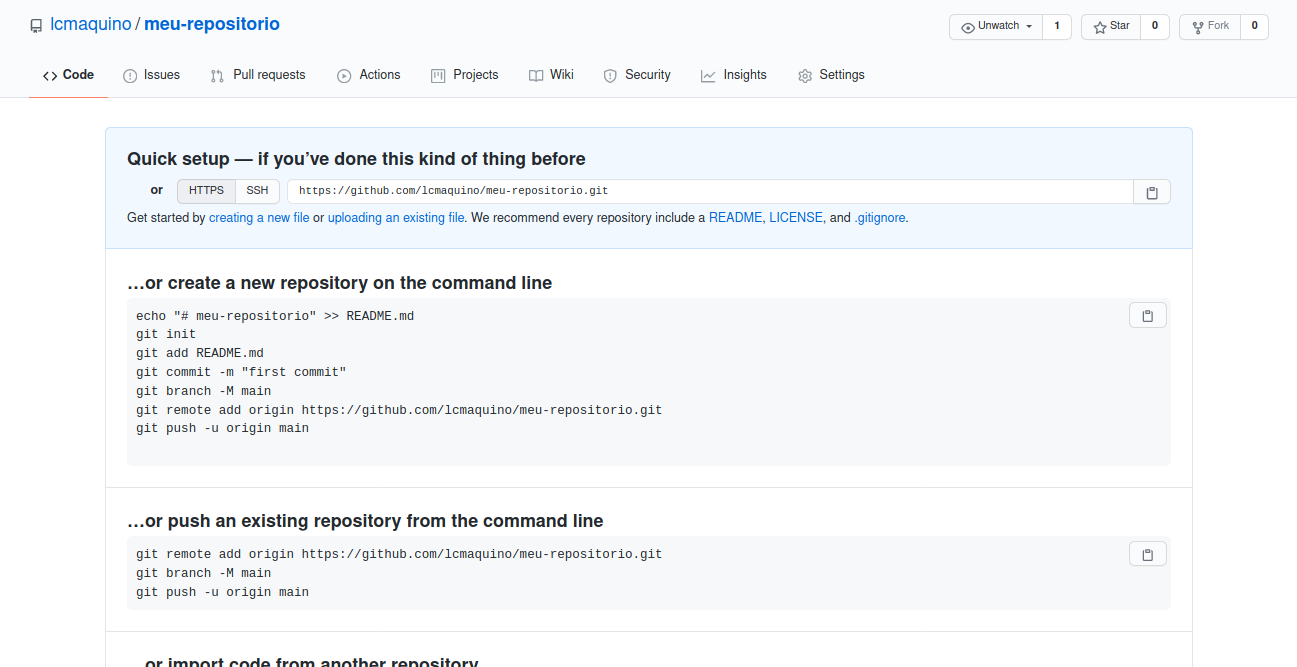
\includegraphics[scale=0.3]{imagens/novo-repositorio-github-3}
\end{figure}
\end{frame}

\begin{frame}{Adicionar o repositório remoto.}

  Vamos adicionar o link do nosso repositório remoto.

  \begin{exampleblock}{Terminal}
    \~\,\$ \terminal{git remote add origin https://github.com/lcmaquino/meu-repositorio.git}
  \end{exampleblock}

  Vamos verificar os links adicionados.

  \begin{exampleblock}{Terminal}
    \~\,\$ \terminal{git remote -v}

    meu-repositorio	https://github.com/lcmaquino/meu-repositorio.git (fetch)

    meu-repositorio	https://github.com/lcmaquino/meu-repositorio.git (push)

  \end{exampleblock}
  
\end{frame}

\begin{frame}{Criar o ramo (\textit{branch}) principal.}

  Vamos criar o ramo ``main'' no nosso repositório.

  \begin{exampleblock}{Terminal}
    \~\,\$ \terminal{git branch -M main}
  \end{exampleblock}
  
\end{frame}

\begin{frame}{Empurrar as mudanças.}

  Vamos empurrar as mudanças para o repositório remoto.

  \begin{exampleblock}{Terminal}
    \~\,\$ \terminal{git push -u origin main}

    Username for 'https://github.com': lcmaquino

    Password for 'https://lcmaquino@github.com':

    Counting objects: 3, done.

    Delta compression using up to 4 threads.

    Compressing objects: 100\% (2/2), done.

    Writing objects: 100\% (3/3), 262 bytes | 262 KiB/s, done.

    Total 3 (delta 0), reused 0 (delta 0)

    To https://github.com/lcmaquino/meu-repositorio.git

    * [new branch] main -$>$ main

    Branch 'main' set up to track remote branch 'main' from 'origin'.
  \end{exampleblock}

\end{frame}

\begin{frame}{Empurrar as mudanças.}

Vamos visualizar nosso repositório remoto.

\begin{figure}
 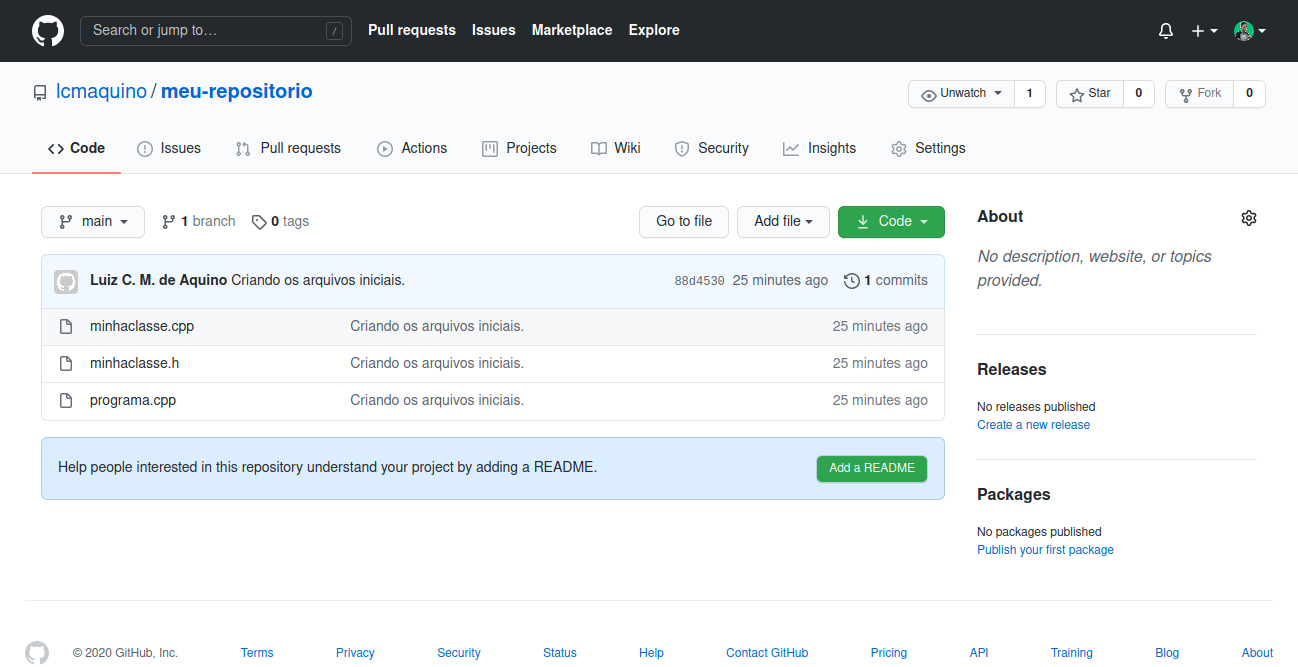
\includegraphics[scale=0.3]{imagens/novo-repositorio-github-4}
\end{figure}
\end{frame}

\begin{frame}{Criar um ramo (\textit{branch}).}

  Vamos criar o ramo ``ramo-teste'' no nosso repositório.

  \begin{exampleblock}{Terminal}
    \~\,\$ \terminal{git branch -M ramo-teste}
  \end{exampleblock}

  Em seguida, vamos ``entrar'' nesse ramo.

  \begin{exampleblock}{Terminal}
    \~\,\$ \terminal{git checkout ramo-teste}

    Switched to branch 'ramo-teste'
  \end{exampleblock}
  
\end{frame}

\begin{frame}{Adicionar um arquivo no ramo.}

Vamos adicionar o arquivo ``readme.txt'' no ramo.

\begin{exampleblock}{Terminal}
\~\,\$ \terminal{git add readme.txt}
\end{exampleblock}

Em seguida, salvar esta mudança.

\begin{exampleblock}{Terminal}
\~\,\$ \terminal{git commit -m ``Adicionar o readme.txt''}

[ramo-teste 937aa51] Adicionar o readme.txt

1 file changed, 1 insertion(+)

create mode 100644 readme.txt
\end{exampleblock}

\end{frame}


\begin{frame}{Empurrar o ramo.}

\begin{exampleblock}{Terminal}
\~\,\$ \terminal{git push -u origin ramo-teste}

Username for 'https://github.com': lcmaquino

Password for 'https://lcmaquino@github.com': 

Counting objects: 3, done.

Delta compression using up to 4 threads.

Compressing objects: 100\% (2/2), done.

Writing objects: 100\% (3/3), 304 bytes | 0 bytes/s, done.

Total 3 (delta 1), reused 0 (delta 0)

remote: Resolving deltas: 100\% (1/1), completed with 1 local object.

To https://github.com/lcmaquino/meu-repositorio.git

* [new branch] ramo-teste -$>$ ramo-teste
\end{exampleblock}

\end{frame}

\begin{frame}{Mesclar os ramos.}

Vamos mesclar o ramo ``ramo-teste'' com o ``main''.

\begin{exampleblock}{Terminal}
\~\,\$ \terminal{git checkout main}

Switched to branch 'main'
\end{exampleblock}


\begin{exampleblock}{Terminal}
\~\,\$ \terminal{git merge ramo-teste}

Updating ac7efeb..937aa51

Fast-forward

readme.txt | 1 +

1 file changed, 1 insertion(+)

create mode 100644 readme.txt
 
\end{exampleblock}

\end{frame}


\begin{frame}{Mesclar os ramos.}

\begin{exampleblock}{Terminal}
\~\,\$ \terminal{git push origin main}

Username for 'https://github.com': lcmaquino

Password for 'https://lcmaquino@github.com':

Total 0 (delta 0), reused 0 (delta 0)

To https://github.com/lcmaquino/meu-repositorio.git

ac7efeb..937aa51  main -$>$ main
 
\end{exampleblock}
\end{frame}

\end{document}
